\chapter{Proposal}
\thispagestyle{myheadings}

	\section{Introduction and Background}

		As the organizations struggle with demands for storage and processing of their data, they increasingly turn to third parties for outsourcing capabilities.
		A number of companies including Amazon (AWS), Microsoft (Azure) and Google (GCP) offer outsourced database solutions to individuals and other businesses.
		This model is lucrative because not only the clients pay exactly for what they use in terms of pure computational resources, but also the cloud takes care of the entire deployment process, including availability, scalability, replication and, most importantly, security.
		Cloud business model is to provide resources on-demand --- from bare-bones \acrshort{vm} to database-as-a-service products.

		While the cloud providers typically have strict customer data privacy policies and even offer server-side encryption-at-rest services, the clients still have to trust the provider with their plaintext data.
		Server-side encryption-at-rest by definition requires the provider to know the encryption key to manipulate the data, even if the key is ephemeral and is not stored in the cloud permanently.
		Moreover, cloud provider in general, and customer's \acrshort{vm} in particular, may be vulnerable to external attacks --- from snapshot-level attacks, in which the adversary has a copy of the \acrshort{vm} memory, to more devastating persistent attacks, in which the adversary continuously monitors the \acrshort{vm} processes.

		Protecting the private information beyond cloud provider guarantees typically requires encrypting it in a way that preserves the ability to process it.
		A line of research targets securing outsourced database systems, but often achieves protection at a cost of efficiency that is too high for a solution to be viable for practical applications.
		In this prospectus, I will cover the constructions that are used to answer different types of database queries in the outsourced model while providing both provable security and practical efficiency guarantees.

		\subsection{Model}\label{section:proposal:intro:model}

			In this work, I consider \emph{an outsourced database system} model, adapted from \cite{generic-attacks-kellaris} and \cite{epsolute}.

			\subsubsection{Outsourced database model}

				Similar to~\cite{epsolute}, a database is abstracted as a collection of \dataSize{} records \record{}, each with a unique identifier \recordID{}, associated with search keys \searchKey{}: \databaseDef{}.
				All records are assumed to have an identical fixed bit-length, and the search keys are elements of some domain \searchKeyDomain{}.
				A query is modeled as a predicate $\query \in \querySet: \searchKeyDomain \to \bin$.
				Evaluating a query \query{} on a database \database{} results in $\query( \database ) = \{ \record_i : \query( \searchKey_i ) = 1 \}$, all records whose search keys satisfy \query{}.

				Formally, an outsourced database system consists of two protocols between a stateful user \user{}, who owns the data, and an untrusted stateful server \server{}, to whom these data are outsourced.
				In setup protocol \protocolSetup{}, \user{} receives as input a database \databaseDef{} and \server{} may optionally output a data structure \serverDS{}.
				In query protocol \protocolQuery{}, \user{} receives a query $\query \in \querySet$, \server{} receives \serverDS{} produced in the setup protocol, and \user{} outputs the result of the query $\query( \database )$.
				Both parties may update their internal states.
				We call a system \emph{correct} if it holds with overwhelming probability over the randomness of the above runs that running \protocolSetup{} and  \protocolQuery{} on the corresponding inputs yields the correct result $\{ \record_i : \query( \searchKey_i ) = 1 \}$.

			\subsubsection{Security model}

				I define two types of adversaries --- a \emph{snapshot} and a \emph{persistent} adversaries.

				A snapshot adversary, as the name suggests, can see a ``snapshot'' of server's data at multiple points in time.
				One can think of such attack as if someone steals a hard drive or accesses a backup.
				Formally, \adversary{} knows \server{} state at all stages of the protocol.

				A persistent adversary is stronger in that she monitors the server continuously.
				Therefore, she can see what snapshot adversary can plus the network traffic and the access pattern.
				Such adversary can be thought of as a malicious software (virus) that runs as a background process with wide permissions.
				Formally, on top of \server{} state, \adversary{} knows the size and content of \server{} communication and the sequence of accesses \server{} makes to its internal state at all stages of the protocol.

				Intuitively, one can think that encrypting records should protect the data.
				Depending on the way the records are encrypted (i.e., whether the semantic or property-preserving encryption is used), this approach can mitigate the snapshot adversary.
				Persistent adversary, however, can observe the communications size even if the traffic itself is encrypted, and can see the access pattern even if the records are protected.
				It has been shown that the knowledge of access pattern~\cite{multidimensional-range-queries, inference-attack-islam-14, leakage-abuse-attacks-cash-15, inference-attacks-naveed-15, generic-attacks-kellaris, attacks-tao-of-inference, grubbs-attacks, access-pattern-disclosure, attacks-improved-reconstruction} or communication volume~\cite{generic-attacks-kellaris, state-of-uniform, attacks-improved-reconstruction, pump-volume-attacks, volume-range-attacks} alone can enable a series of reconstruction attacks.
				Also note that both adversaries are \emph{honest-but-curios} --- they only observe and never interfere.
				Denial-of-service attacks and integrity protection are out of scope of this work.

			\subsubsection{Query types}

				The type of query \query{} is deliberately left abstract.
				The outsourced database system assumes that a query contains a way (a predicate) to select only the records whose search keys satisfy it.
				In this work I consider these types of queries.

				\paragraph*{A point query.}
					This query selects records whose key is equal to a certain value.
					The domain of the point value does not have to be ordered; it can be categorical, like color names.
					The relevant SQL query can be

					\texttt{SELECT * FROM t1 WHERE zip = '02215'}.

				\paragraph*{A range query.}
					This query selects records whose key lies between two values from an ordered domain.
					The relevant SQL query can be

					\texttt{SELECT * FROM t1 WHERE age BETWEEN 18 and 65}.

				\paragraph*{A \knn{} query.}
					$k$-nearest neighbor query selects $k$ records whose keys are ``closest'' to a certain value.
					This query type requires a definition of distance metric over the domain of search keys, for example, simple Euclidean distance.
					The relevant SQL query can be

					\texttt{SELECT * FROM t1 ORDER BY location <-> '(29.9691,-95.6972)' LIMIT 5}. % chktex 36

		\subsection{Proposal}

			I propose to structure the thesis around the problem of answering the aforementioned three query types securely in the presence of snapshot or persistent adversaries.
			The thesis will include a rich background on proposed secure query processing solutions and attacks against these solutions.
			I will explain the components that are needed to construct the solutions, including symmetric encryption, property-preserving encryption, \acrlong{oram} and Differential Privacy.

	\section{Range queries in a snapshot model}

		\subsection{Problem}

			There are a plenty of works offering range query solutions in a snapshot adversary model.
			Some authors propose a new \acrfull{ore} scheme to be used inside an existing range query index, see \cite{bclo-ope,clww-ore,lewi-wu-ore,cloz-ore,fh-ope}.
			Others suggest full client-server protocols with different security guarantees, see \cite{florian-protocol,pope,practical-ore}.

			Instead of adding another solution to the mix, we developed a robust evaluation framework to compare and audit different \acrshort{ore} schemes and range query protocols \cite{ore-benchmark-17}.
			We have noticed that all proposed solutions offer their own formal protocol, security definition (which they obliviously satisfy), and even performance metrics.
			Moreover, only a few of these algorithms have ready-to-use open-sourced code.
			More often, the implementation is a prototype (or does not even exist), rendering experiments non-reproducible.

		\subsection{Solution}

			Our work addresses these shortcomings.
			We proposed a common framework where all analyzed solutions follow the same formal protocol, a variant of outsourced database from \cref{section:proposal:intro:model}.
			The schemes and protocols are also tested against the same security definition, a variant of simulation-based security game where simulator has a leakage function that is different for each solution.
			Lastly, all protocols are implemented in the same language and runtime, and are using the same cryptographic primitive implementations.

			We have paid extra attention to how we quantify the performance.
			Published works typically claim that they have implemented the algorithm in some language and ran it on a server many times measuring the wall-clock time.
			Such metric is deeply flawed since it only measures just that --- the wall-clock time it took for a particular machine to execute a particular code that references particular implementations of primitives and makes (or even does not make) \IO{} requests to particular hardware.
			What we offer is a metric that drops all these ``particulars'' (i.e., dependencies) from the protocol execution.
			On top of having all solutions implemented in the same language and using same primitives, instead of measuring the time we count the number fo times an \acrshort{ore} scheme makes use of a primitive and a protocol makes an \IO{} request.
			This metric is much more demonstrative: one can always get a wall-clock time estimate given these counts and the specs of the hardware.
			Moreover, we can analyze these counts theoretically from the pseudocode and then verify them practically after running the code.

		\subsection{Results}

			In our work we apply the framework to ten range query solutions.
			Five protocols are built with an \acrfull{ore} scheme coupled with a \BPlus{} tree.
			In \protocolSetup{}, \client{} encrypts all search keys with the \acrshort{ore} scheme, constructs a \BPlus{} tree from the ciphertexts and uploads to \server{}.
			In \protocolQuery{}, \client{} sends encrypted query endpoints and \server{} follows standard \BPlus{} traversal.
			Such protocol leaks the total order of the records plus the leakage of the underlying \acrshort{ore} scheme.

			We also analyzed dedicated range query protocols from \cite{florian-protocol,pope,practical-range-search} and two more baselines.
			Baselines are chosen at the extremes of performance / security spectrum --- a plaintext \BPlus{} tree and a \BPlus{} tree in \acrshort{oram}.
			Intuitively, all solutions should lie between the baselines in both performance and security, but we show that at least performance-wise it is not the case (see one of the plots in \cref{figure:ore}).

			Please see \cref{table:ore,table:range} in \cref{appendix:ore-results} for the analytical results for each solution, and \cite{ore-benchmark-17} for experimental results.

			\begin{figure}[h]
	\centering
	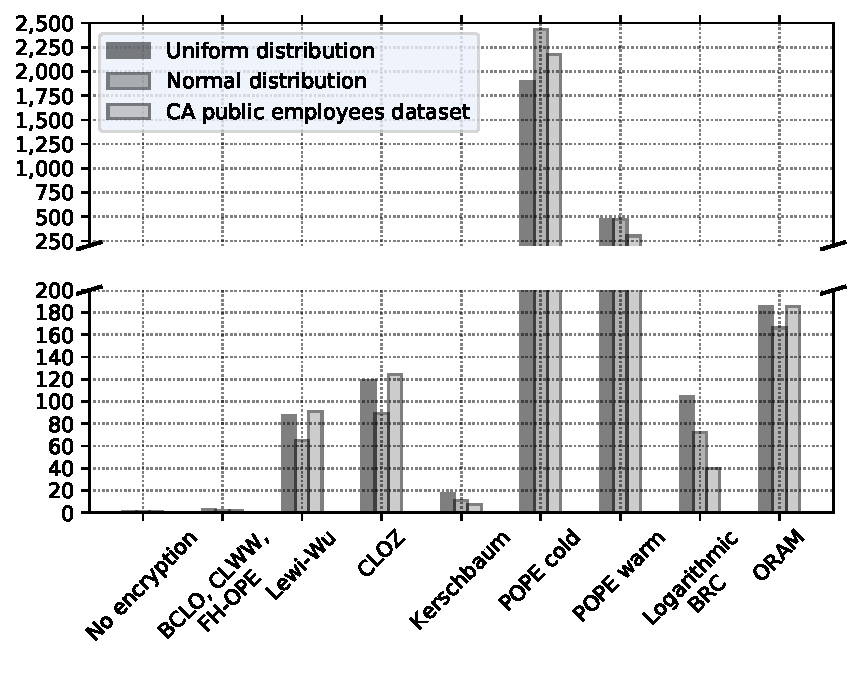
\includegraphics[width=1.0\textwidth]{protocol-charts-qios}
	\caption{Query stage number of I/O requests \cite[Figure 2d]{ore-benchmark-17}}\label{figure:ore}
\end{figure}


	\section{Range and point queries in a persistent model}\label{section:range-queries-persistent}

		\subsection{Motivation and Background}

			A persistent adversary is capable of observing not only the data at any point in time (like the snapshot attacker), but also all processes and communication on the server, including the network messages, their size and the access pattern to the storage.
			A series of attacks starting with a seminal work of \textcite{generic-attacks-kellaris} showed that the query result size~\cite{generic-attacks-kellaris, state-of-uniform, attacks-improved-reconstruction, pump-volume-attacks, volume-range-attacks} and access pattern~\cite{multidimensional-range-queries, inference-attack-islam-14, leakage-abuse-attacks-cash-15, inference-attacks-naveed-15, generic-attacks-kellaris, attacks-tao-of-inference, grubbs-attacks, access-pattern-disclosure, attacks-improved-reconstruction} alone can enable reconstruction attacks.
			The attacks against access pattern typically exploit the fact that some records are accessed more often that others and in the same query as others.
			The adversary maps this knowledge to some public auxiliary dataset and queryset and guesses the values correctly with a non-negligible probability.
			Attacks on communication volume are more elaborate and use the fact that there are a well-defined number of distinct interval queries over the domain.
			\textcite{generic-attacks-kellaris}, for example, construct a polynomial with the observed number of queries that return different number of records, and solve it deriving the exact reconstruction.

			Generic way to protect the access pattern is the \acrfull{oram}, an interactive client-server protocol that conceals the access pattern from the observing adversary by making at least $\bigO{\log n}$ extra requests.
			A na\"{\i}ve solution is to simply proxy all requests through the \acrshort{oram} protocol, but it is generally inefficient and not trivially parallelizable.

			Protecting against communication volume leakage usually involves returning a number of extra fake records and letting the client filter them out locally.
			Where approaches differ is in the number of these fake records.
			A na\"{\i}ve way of adding a constant amount of noise or even sampling noise uniformly is insecure since such noise can be filtered out by the adversary either immediately (constant noise), or after observing a certain number of queries (uniform noise).
			Another dimension to the problem is how much noise to add to have a provable guarantee and yet add the smallest amount of noise possible.

			\subsubsection{Differential Privacy}

				The most effective approach is sampling noise using \acrfull{dp}.
				\acrshort{dp} is a guarantee on a query algorithm that takes a database and returns some result.
				The guarantee states that for two neighboring databases (that differ in one record), probability that the adversary will understand by looking at the output, which of the two databases was used as an input, is bounded.
				More formally, the \acrshort{dp} is defined in \cref{definition:dp}.

				\begin{definition}[Differential Privacy, adapted from~\cite{our-data-ourselves, differential-privacy-original}]\label{definition:dp}
					A randomized algorithm \algo{A} is $(\epsilon, \delta)$-differentially private if for all $\database_1 \sim \database_2 \in \searchKeyDomain^\dataSize$, and for all subsets $\mathcal{O}$ of the output space of \algo{A},
					\[
						\probability{ \algo{A}{ \database_1 } \in \mathcal{O} } \leq \exp(\epsilon) \cdot \probability{ \algo{A}{ \database_2 } \in \mathcal{O} } + \delta \; .
					\]
				\end{definition}

				One way to make sense of this definition is the following.
				Probabilities are taken over the coins of algorithm \algo{A}, which answers a query based on a dataset.
				A natural instantiation of \algo{A} is a view of a distinguishing adversary \adversary{}, who tries to guess which of the two datasets was used.
				The expression in \cref{definition:dp} then bounds the advantage of \adversary{} with $\epsilon$ and $\delta$ parameters.
				Note that $\exp( x ) \approx 1 + x + \frac{x^2}{2!}$ and for sufficiently small $x$ the last term is negligible.
				If we put $\epsilon + 1$ in place of $\exp( \epsilon )$, it becomes clear that $\epsilon$ is the exact value by which two probabilities are allowed to differ.
				For $\epsilon = 0$, they have to be equal, for $\epsilon = 0.01$, probabilities may differ by \SI{1}{\percent}.
				Therefore, $\epsilon$ is called \emph{a privacy budget} of a \acrshort{dp} system.
				$\delta$ term is additive and therefore must be small by itself.
				This term is essentially a probability that the entire system fails, for example, if \algo{A} is a randomized algorithm which fails with a certain chance, this probability will be $\delta$.
				For instance, a PathORAM \cite{path-oram} algorithm can have a stash overflow with a bounded probability \cite[Theorem 1]{path-oram} and it will cause the entire algorithm to fail.
				If PathORAM is used in a \acrshort{dp} system then this probability, however small, bounded and negligible, will have to be accounted for in $\delta$.

				Note that \cref{definition:dp} describes a property of \algo{A} and not a construction method.
				To construct \algo{A}, the seminal \cite{differential-privacy-original} offers an algorithm called \acrfull{lpa}.
				The idea is to tune the noise sampled from Laplacian distribution to the \emph{sensitivity} of a query, defined as the change of output with respect to change in input.
				For example, if a change in one record of the dataset causes a change in the output value of at most one (e.g., a count query), then the sensitivity is 1.
				\cite{differential-privacy-original} proves that if one adds $\algo{Laplace}{0, \frac{\mathsf{sensitivity}}{\epsilon}}$ to the real result of a query, the resulting mechanism is $\epsilon$-\acrshort{dp}.

				Lastly, instead of generating and adding noise each query, it is possible to generate noisy values once, embed them into the data and release the sanitized data without compromising privacy guarantees.
				The intuition is that once the noise is embedded in the dataset, adversary can run a regular query over it and the entire query will still be \acrshort{dp}.
				Such methods are collectively called \emph{sanitization}, and there are known bounds for point and range queries, for pure ($\delta = 0$) and approximate ($\delta > 0$) \acrshort{dp} \cite{bounds-on-sample-complexity,private-learning-and-sanitization,non-interactive-database-privacy,dp-under-observation,dp-release,privately-learning-thresholds}.

		\subsection{Security definition}

			In this work we aim for the most practical definition of security, which needs to capture both access pattern and communication volume protection and yet be feasible enough so that an efficient system exists that can satisfy it.
			In \epsolute{} \cite{epsolute} we propose a definition of computationally \acrshort{dp} outsourced database.

			\begin{definition}[\acrfull{cdpodb} from Definition 3.1 in \cite{epsolute}]\label{definition:cdpodb}
				We say that an outsourced database system \protocol{} is $(\epsilon, \delta)$-computationally differentially private (a.k.a.\acrshort{cdpodb}) if for every polynomial time distinguishing adversary \adversary{}, for every neighboring databases $\database \sim \database^\prime$, and for every query sequence $\fromNtoM{\query}{1}{m} \in \querySet^m$ where $m = \mathsf{poly}(\lambda)$,

				\begin{multline*}
					\probability{\adversary \left( 1^\lambda, \view{\protocol, \server}{\database, \fromNtoM{\query}{1}{m}} \right) = 1 } \leq \\
					\exp{\epsilon} \cdot \probability{\adversary \left( 1^\lambda, \view{\protocol ,\server}{\database^\prime, \fromNtoM{\query}{1}{m}} \right) = 1} + \delta + \negl \; ,
				\end{multline*}
				the probability is over the randomness of the distinguishing adversary \adversary{} and the protocol \protocol{}.
			\end{definition}

			First thing to note in this definition is that unlike in prior works where only a part of \adversary{}'s view is \acrshort{dp}-protected (e.g., only access pattern in \cite{differential-obliviousness,differential-obliviousness-followup}), here the entire view of the adversary is protected.
			That is, if \emph{anything} that is visible during the protocols execution to a persistent adversary can be used to distinguish the neighboring datasets, the adversary wins and the system fails to satisfy the definition.
			Subsequently, it implies protection against both access pattern and communication volume, since they are both a part of the view and if adversary sees either of them, she can distinguish.

			Also note that the \acrshort{cdpodb} system is \acrshort{dp}, but not necessarily semantically secure.
			A semantically secure database would have had probabilities almost equal (or, in \cref{definition:cdpodb}, $\epsilon = 0$).
			The trade-off has been made to allow a construction of an efficient system.
			While a na\"{\i}ve solution that satisfies semantically secure definition would return entire dataset every query, constructing a practical instantiation is hard, is not necessarily possible, and remains an open problem.

			The negligible term $\negl$ at the end was added to account for computational (as opposed to information-theoretical) nature of the definition.
			In information-theoretical system the security is guaranteed by the clear mathematical proof that the adversary can do nothing better than brute-force the system (e.g., iterating over one-time-pad keys).
			A computational security definition relies on the fact that the adversary simply does not have enough resources to break a system, which may or may not hold true in the future.
			For example, the problems of finding a discrete logarithm and factorization are only assumed to be hard, as are standardized block ciphers, such as AES \cite{aes-nist}.
			Therefore, if we want to allow a system to use these cryptographic blocks for security, we must include it in the definition.

			Finally, note the query sequence $\fromNtoM{\query}{1}{m} \in \querySet$ is fixed.
			The definition is non-adaptive in a sense that the user \user{} must not choose the next query based on the result of the previous one.
			In \cite[Section 3.1.1]{epsolute} we prove by example why this limitation is inherent and an no efficient system can be built that allows adaptive queries.

		\subsection{\epsolute{}}

			In \epsolute{} \cite{epsolute}, we develop a method of answering point and range queries that satisfies \cref{definition:cdpodb}.
			In the heart of the construction is using \acrshort{oram} to hide access pattern and \acrshort{dp} to add extra fake records to the result to hide communication volume.

			\acrshort{oram} component is straightforward --- communication between \user{} and \server{} is routed thorough the \acrshort{oram} protocol.
			This approach, however, substantially increases the overhead, which I will will address in \cref{section:range-queries-persistent:parallel-epsolute}.

			To properly and optimally add noise to the true result we make use of sanitizers for point and range query types.
			For point queries, we construct a histogram from the domain values.
			We put the number of records for the domain value plus the noise sampled from the Laplacian distribution into each bin.

			\begin{figure}[h]
	\centering
	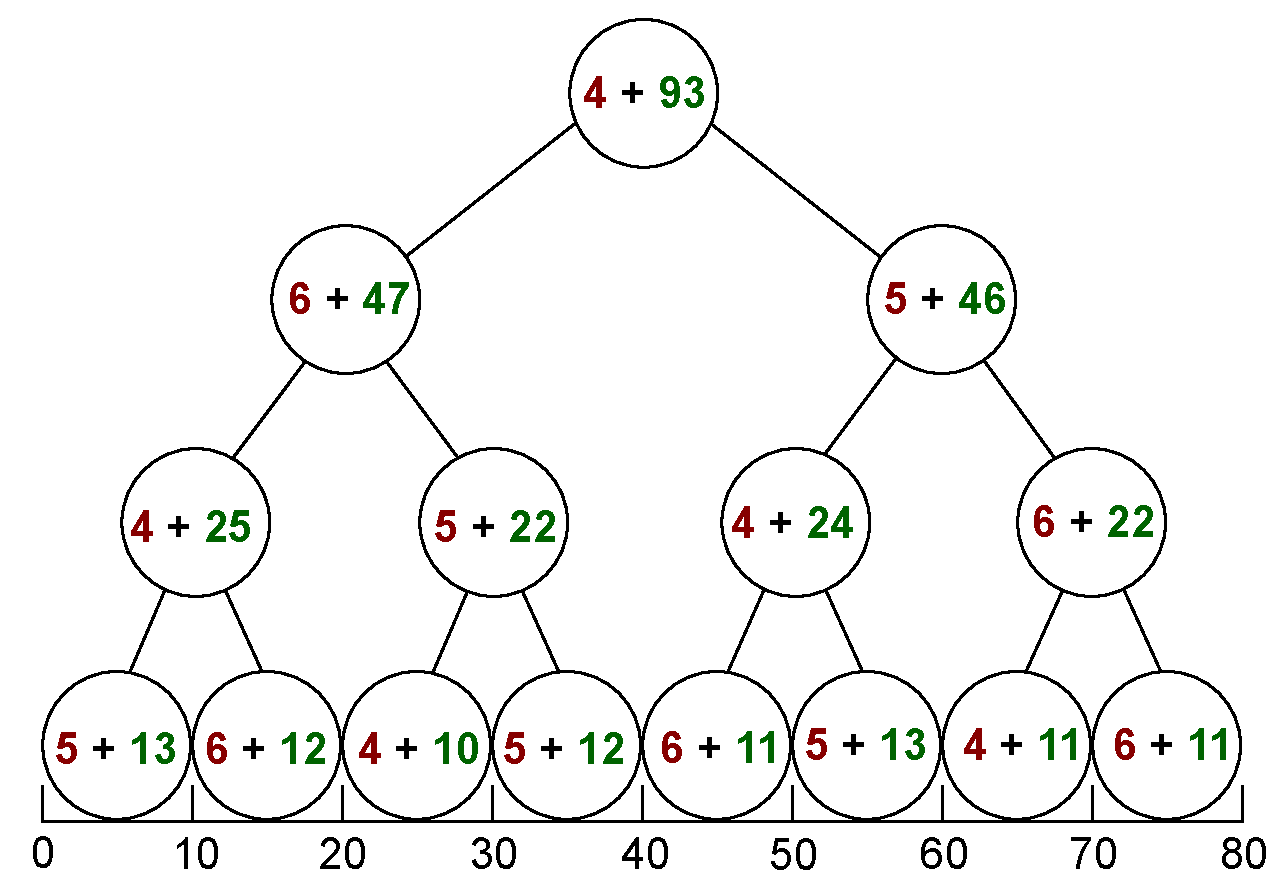
\includegraphics[width=1.0\textwidth]{sanitizer}
	\caption[An example of a hierarchical sanitizer]{
		An example of a hierarchical sanitizer \cite{hierarchical-methods-for-dp} with fanout $\fanout = 2$.
		Left (red) value is noise and right (green) value is the number of records covered by the node.
		To answer a query $[3, 28]$, we take only two nodes $(4 + 25)$ and $(4 + 10)$ with a resulting noise of 8 and 35 real records.
	}\label{figure:sanitizer}
\end{figure}


			For the range queries we use a hierarchical sanitizer \cite{hierarchical-methods-for-dp}, see example on \cref{figure:sanitizer}.
			We first split continuous domain into bins.
			Then we build a \fanout{}-ary tree over domain bins and put the number of records plus noise into each node.
			The leaves get values same way as in histogram, and intermediate node value is a sum of counts of all records in all children bins plus a single noise sample.
			Compared to plain histogram, this construction has a benefit that if the range is wide we can answer the query using only the intermediate node and not all leaf nodes.
			Since each bin is now associated with $\ceil{\log_\fanout B}$ nodes, where $B$ is the number of bins, we amplify our noise respectively.

			Note that the Laplacian distribution is symmetrical and unbounded, so if we sample from a zero-mean distribution some of the samples will be negative.
			Since we do not allow negative noise and since na\"{\i}vely truncating the distribution will break \acrshort{dp} guarantees, we need to shift the mean of the distribution.
			Doing so will only increase the noise thereby maintaining the guarantees.
			We have analytically derived the smallest mean of the distribution to ensure that the samples are non-negative for the entire histogram or tree with a set probability $\delta$.
			These values are
			\[
				\mu_{\mathsf{point}} = \ceil{ -\frac{ \ln \left( 2 - 2 \sqrt[\domainSize]{1 - \delta} \right) }{ \epsilon } } \quad \text{and} \quad \mu_{\mathsf{range}} = \ceil{ -\frac{ \ln{ (2 - 2 \sqrt[\mathsf{nodes}]{ 1 - \delta } ) } \cdot \log_{\fanout} \domainSize }{\epsilon} }
			\]
			for domain size \domainSize{} and the number of nodes in a tree $\mathsf{nodes}$.

			With this prerequisites we construct the actual setup and query protocols.
			See visualization of \protocolQuery{} in \cref{figure:epsolute}.
			\begin{itemize}
				\item
					Setup protocol \protocolSetup{}
					\begin{enumerate}
						\item
							On input a dataset \database{}, \user{} creates and keeps locally an inverted index over the records mapping the search keys \searchKey{} to record IDs \recordID{}.
						\item
							\user{} and \server{} engage into the \acrshort{oram} protocol, where \user{} is a client.
							\user{} stores all records by their IDs.
						\item
							\user{} constructs a sanitized structure \serverDS{}, a \acrshort{dp}-histogram for point queries or a \acrshort{dp}-tree for range queries, over the domain of the dataset and posts it to \server{}.
					\end{enumerate}
				\item
					Query protocol \protocolQuery{}
					\begin{enumerate}
						\item
							On input a query \query{}, \user{} looks up record IDs in its local index.
						\item
							\user{} requests \serverDS{} from \server{} and uses it to calculate the total number of requests $c$ (the number of true records for the query plus noise).
						\item
							\user{} and \server{} engage into the \acrshort{oram} protocol, where \user{} is a client.
							\user{} loads $c$ records where these requests include all true records and the rest are random and non-repeating.
						\item
							\user{} prunes the fake records and returns the true ones.
					\end{enumerate}
			\end{itemize}

			\begin{figure}[h]
	\centering
	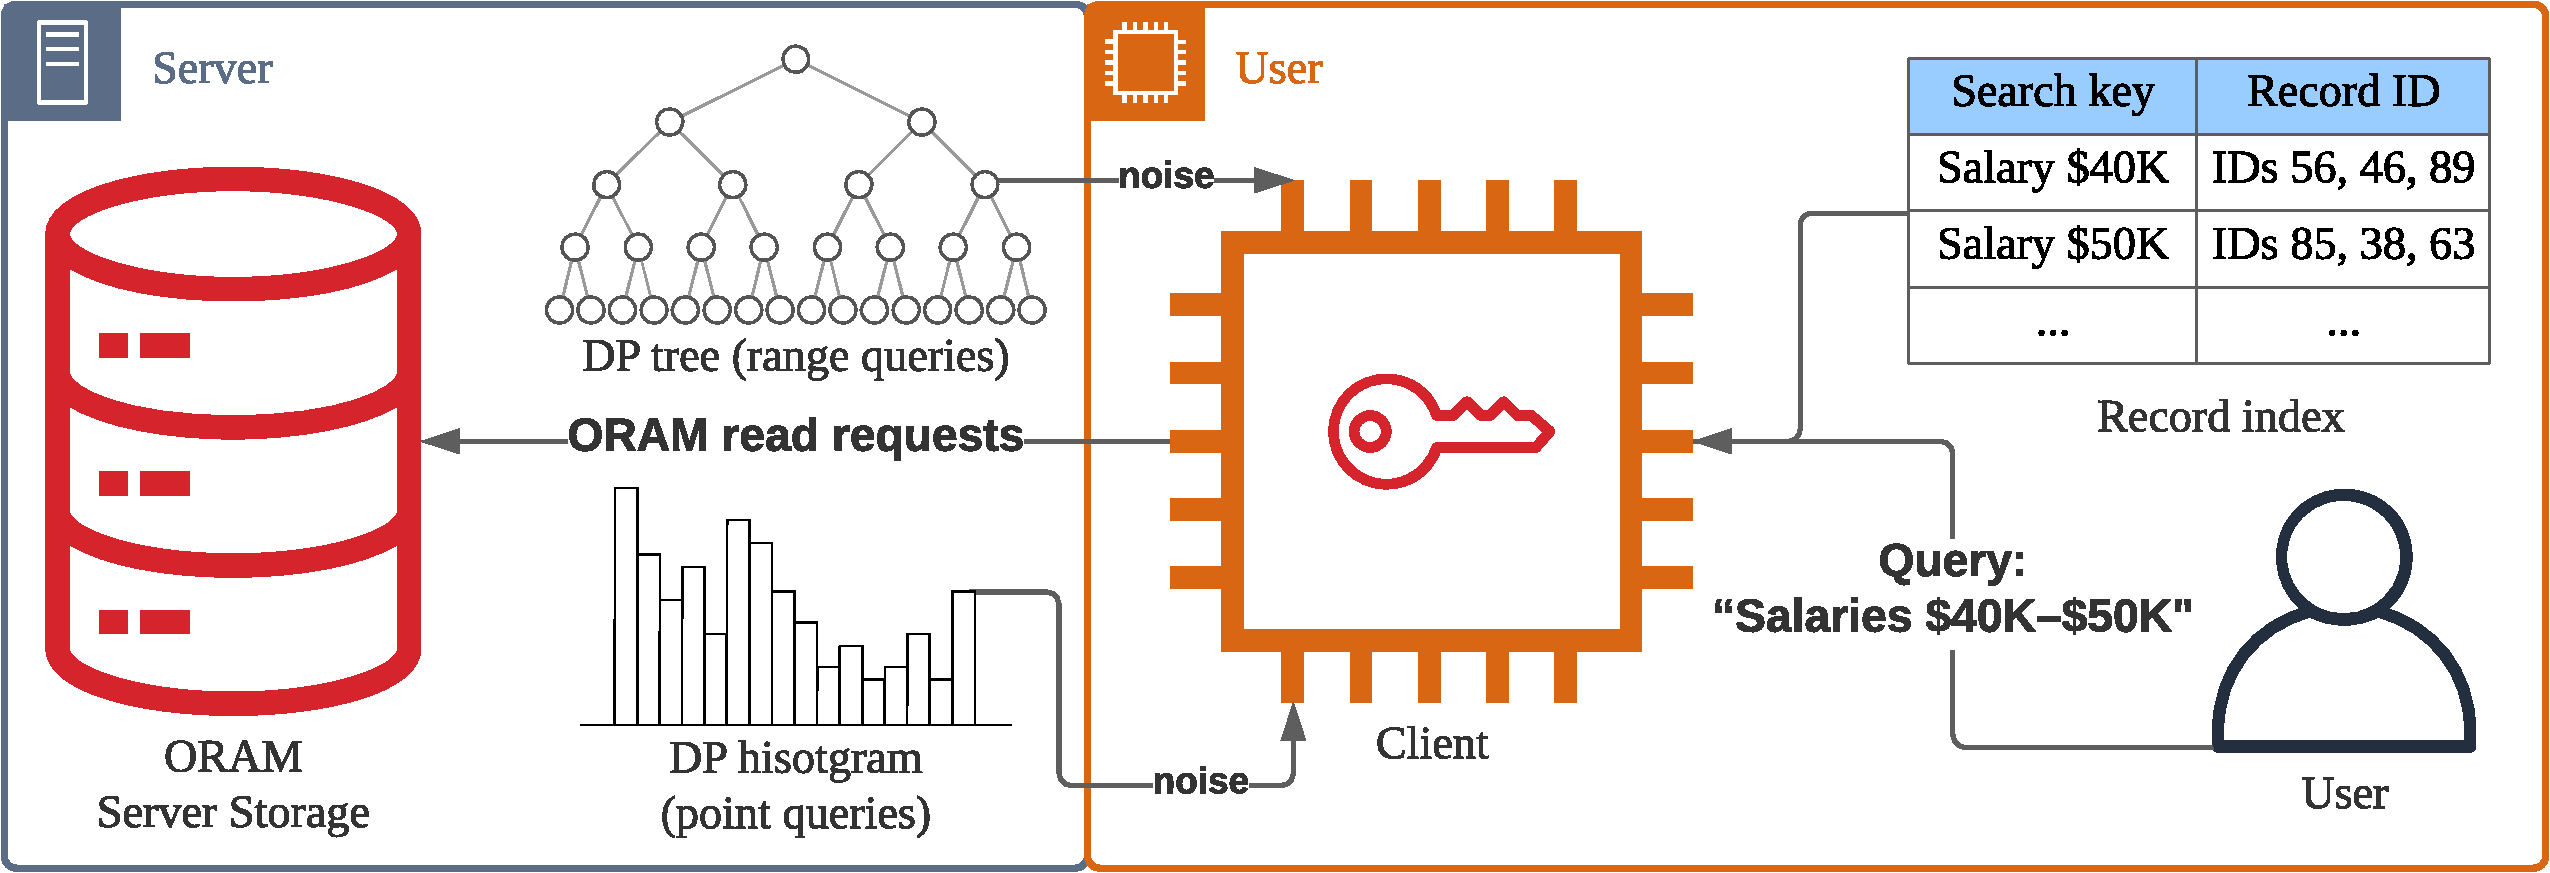
\includegraphics[width=1.0\textwidth]{epsolute}
	\caption{Query protocol \protocolQuery{} of \epsolute{}.}\label{figure:epsolute}
\end{figure}


			This method, to which I will refer to as \emph{a single-threaded \epsolute{}}, is a \acrlong{cdpodb} as defined in \cref{definition:cdpodb}, see proof in \cite[Section 4.2]{epsolute}.

		\subsection{Parallel \epsolute{}}\label{section:range-queries-persistent:parallel-epsolute}

			While the single-threaded \epsolute{} is an efficient \acrshort{cdpodb} in sense that it returns only a fraction of total records per query, it is still slow in practice because of the $\bigO{\log \dataSize \log \domainSize}$ overhead due to \acrshort{oram} and \acrshort{dp}-sanitizer.
			To bring the construction closer to real-world demands in performance we devise a parallel solution.

			\subsubsection{A choice of separate vs shared sanitized dataset}

				A natural approach is to split the dataset \database{} into \oramsNumber{} partitions and run parallel \acrshort{oram} protocols against a distributed \server{}.
				The partitioning part is not hard --- we split records by the hash of their unique ID and we construct smaller (and thus logarithmically faster) \acrshortpl{oram} over the partitions along with \oramsNumber{} inverted indices on \user{}.
				However, we need to decide how we sample \acrshort{dp} noise in this setting.
				The two approaches are generating a separate \serverDS{} per partition or using a shared \serverDS{}.

				When generating a separate \acrshort{dp}-sanitized dataset \serverDS{} per partition there are two competing effects on performance.
				On the one hand, each thread on average returns a \nicefrac{1}{m} fraction of the result from an \acrshort{oram} with overhead $\log \frac{n}{m}$.
				On the other hand, each thread now adds independent noise, which results in \oramsNumber{} amplification of noise.
				Moreover, due to \acrshort{dp} composition theorem \cite{privacy-integrated-queries,differential-privacy-original,our-data-ourselves} for disjoint datasets, the privacy budget of the system is the privacy budget of the least private component.
				Since we cannot assume that the distribution of resulting records in all queries is always uniform, we bound a worst-case scenario of a single \acrshort{oram} having most of the result records.
				In \cite[Section 5.1]{epsolute} we have found that the noise is amplified by an extra $\left( 1 + \sqrt{ \frac{-3 m \log \delta}{k_0} } \right)$ factor, where $k_0$ is the number of true records for a query.

				When generating a single shared \serverDS{} for all \oramsNumber{} partitions, we need to ensure that the total number of records returned by each thread is the same.
				We reuse the amplification factor from previous approach and set new $\tilde{k}_0 = k_0 + \frac{\log^{1.5} N}{\epsilon}$ for range queries and $\tilde{k}_0 = k_0 + \frac{\log N}{\epsilon}$ for point queries due to the use of \acrshort{dp} sanitizers.
				The total generated noise is now larger but it is now split among \oramsNumber{} threads and it grows slower than linear in \oramsNumber{}.

				Comparing these two methods we conclude that in most cases the shared \serverDS{} is faster (i.e., results in fewer total fetched records), especially for an increasing parallelization factor.
				First, the former method is not guaranteed to have a uniform load among threads.
				In fact, while on average the amount of work per thread may be smaller, there may be a single disproportionally overloaded thread, which would cause the entire system to slow down.
				Second, while the number of true records per thread will decrease linearly for the former method, the noise factor will stay constant and will at larger \oramsNumber{} dominate the amount of work precluding further scalability.
				The latter method is more scalable in this regard since the amount of work decreases linearly while the amount of noise increases only logarithmically with the number of threads.

			\subsubsection{The construction}

				With this analysis I present an upgraded construction, \emph{a parallel \epsolute{}}, see \cref{figure:parallel-epsolute}.
				The core protocol is similar to single-threaded version except some of the operations are distributed and executed in parallel.
				\begin{itemize}
					\item
						Setup protocol \protocolSetup{}
						\begin{enumerate}
							\item
								On input a dataset \database{}, \user{} partitions it into \oramsNumber{} segments \fromNtoM{\database}{1}{\oramsNumber} by a hash of record IDs \recordID{}.
								\user{} then creates and keeps locally \oramsNumber{} inverted indices over the records mapping the search keys \searchKey{} to record IDs \recordID{} in a respective partition.
							\item
								\user{} and distributed \server{} engage into \oramsNumber{} \acrshort{oram} protocols, where \user{} is a client.
								\user{} stores all records by their IDs in respective \server{} partitions.
							\item
								\user{} constructs a sanitized structure \serverDS{} (or \oramsNumber{} such structures depending on the choice of method) over the domain of the dataset and posts it to \server{}.
						\end{enumerate}
					\item
						Query protocol \protocolQuery{}
						\begin{enumerate}
							\item
								On input a query \query{}, \user{} looks up record IDs in its local indices.
							\item
								\user{} requests \serverDS{} (one or multiple) from \server{} and uses it to calculate the total number of requests $c$.
								Depending on the choice of method, \user{} prepares a sequence of requests to \server{}.
							\item
								\user{} and \server{} engage into \oramsNumber{} \acrshort{oram} protocols, where \user{} is a client.
								\user{} loads a total of $c$ records where these requests include all true records and the rest are random and non-repeating.
							\item
								\user{} waits for the last thread to finish, prunes the fake records and returns the true ones.
						\end{enumerate}
				\end{itemize}

				As a purely practical optimization, instead of making a single client \acrshort{vm} engage into \oramsNumber{} (up to 128 in the experiments) connections and heavy cryptographic threads, we logically split \user{} into a principal \acrshort{vm}, which handles main logic, and a set of helper \acrshortpl{vm} that only engage in a number of \acrshort{oram} protocols.

				\begin{figure}[th]
	\centering
	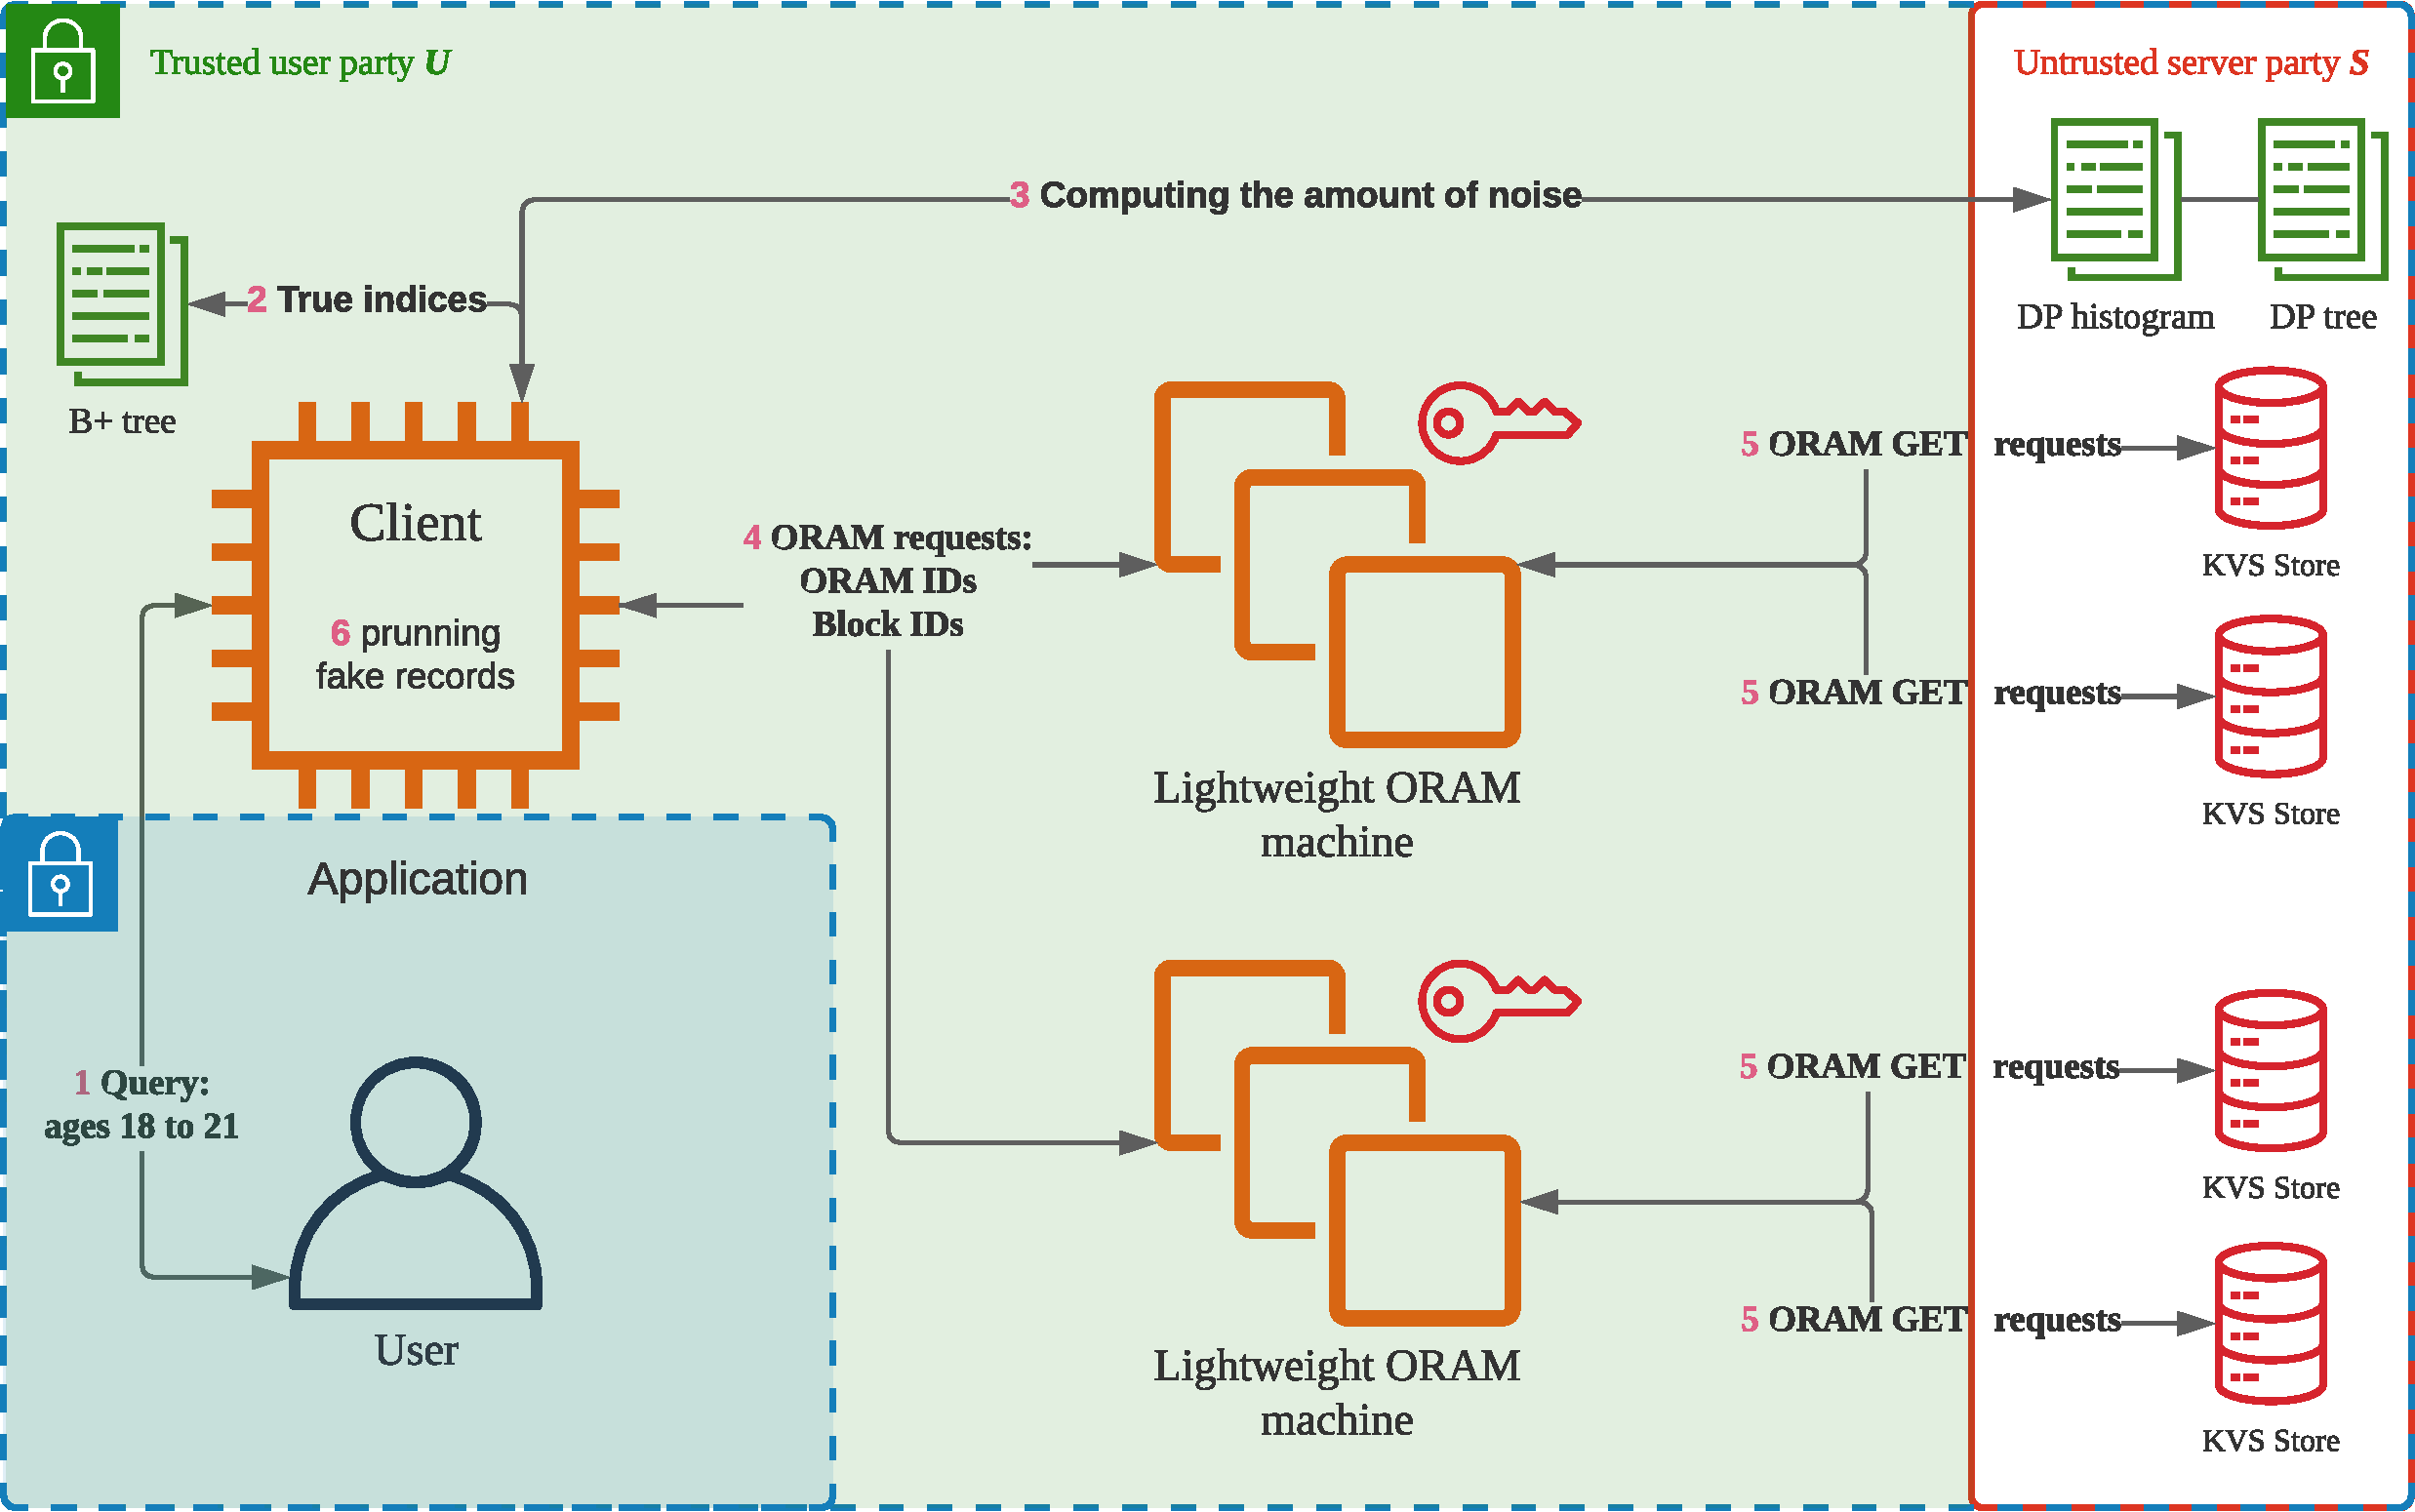
\includegraphics[width=1.0\textwidth]{parallel-epsolute}
	\caption{Query protocol \protocolQuery{} of parallel \epsolute{}.}\label{figure:parallel-epsolute}
\end{figure}


